\section{Evaluation}
\label{sec:Evaluation}

In this section, we provide a detailed overview of the three publicly available datasets utilized in our experiments: DexYCB \cite{chao2021dexycb}, FPHAB \cite{garcia2018first}, and HO-3D \cite{hampali2020honnotate}. Each of these datasets presents unique challenges and characteristics that are essential for evaluating the robustness and accuracy of in-hand object pose tracking methods. We benchmark our approach against state-of-the-art methods across various metrics, including Average Precision (AP) and Area Under the Curve (AUC), showing that our model consistently achieves higher accuracy, particularly in challenging scenarios involving heavy occlusions and rapid hand movements.

\subsection{Datasets}

\textbf{DexYCB Dataset} \cite{chao2021dexycb}. The DexYCB dataset is highly suitable for evaluating hand-held object pose tracking in videos due to its comprehensive set of annotated hand-object interactions. The dataset includes over 582 video sequences capturing the dynamic manipulation of 20 different objects from the YCB dataset by 10 subjects. Each sequence provides 6D object poses, 3D hand poses, and RGB-D data, which are crucial for testing the robustness and accuracy of tracking algorithms in real-world conditions. The variety of objects, coupled with naturalistic hand movements, makes DexYCB an ideal benchmark for assessing how well a model can maintain accurate pose estimates over time, particularly in scenarios involving rapid hand movements and frequent occlusions. To prepare the dataset, we follow the benchmark setup $S0$ (default) as defined in \cite{chao2021dexycb}. The train split contains sequences from all 10 subjects, all 8 camera views, and all 20 grasped objects. We ensure that no sequences are shared between the training, validation, and test splits. Images are resized to $256 \times 256$ pixels, and data augmentation techniques, including random rotation, scaling, and brightness adjustments, are applied during training to enhance model generalization. 

\noindent \textbf{FPHAB Dataset} \cite{garcia2018first}. The First-Person Hand Action Benchmark (FPHAB) dataset is particularly relevant for evaluating pose tracking in first-person view scenarios. It offers 1175 RGB-D video sequences across 45 different action classes, all annotated with 3D hand poses. This dataset is valuable for testing hand-held object pose tracking models because the egocentric viewpoint introduces challenges such as motion blur, self-occlusion, and varying lighting conditions, which are common in real-world applications. By providing a diverse set of actions and interactions, FPHAB enables the assessment of a model's ability to track objects consistently despite the inherent complexities of first-person perspectives. In our setup, the dataset is preprocessed by resizing images to $256 \times 256$ pixels. We split the dataset into approximately 70,000 frames for training and 30,000 frames for testing. Data augmentation, including random flipping, cropping, and color jitter, is applied to the training set. To evaluate the model's robustness to occlusions, more than 70\% of the test set images involve occlusions, with at least 50\% of those under heavy occlusion.

\noindent \textbf{HO-3D Dataset} \cite{hampali2020honnotate}. This dataset is specifically designed to evaluate 3D hand-object pose estimation, making it an excellent benchmark for hand-held object pose tracking in videos. With over 80,000 annotated frames, this dataset captures intricate hand-object interactions, often under challenging conditions like severe occlusions and complex background scenes. The sequences in HO-3D are recorded in real-world environments, providing a realistic testbed for assessing the effectiveness of pose tracking algorithms. The dataset's emphasis on naturalistic hand movements and object manipulation in cluttered environments is critical for evaluating how well a model can maintain accurate pose estimates across frames when faced with partial or full occlusions. We preprocess the dataset by resizing all images to $256 \times 256$ pixels and applying data augmentation such as random rotation, scaling, and brightness adjustments to enhance diversity in the training data. The dataset is split into approximately 65,000 frames for training and 10,000 frames for testing, with over 70\% of the test set images involving occlusions and at least 50\% of those under heavy occlusion.

\subsection{Implementation Details}

Our implementation\footnote{Our code and other materials are available at \url{https://github.com/hoangcuongbk80/6dInHandVid}} employs ResNet-50 \cite{he2016deep} combined with ROIAlign \cite{he2017mask} to extract object features at an output resolution of $32 \times 32$ with 256 feature channels. The spatial transformer module, which includes both the encoder and decoder, is built with 3 layers of multi-head self-attention. Each attention layer contains 8 heads, with a feed-forward network dimension of 256. The transformer decoder uses query vectors with a dimensionality of 256, and the temporal transformer shares the same architecture as the spatial transformer. The ResNet-50 backbone is initialized with ImageNet-pretrained weights, while the transformer components are trained from scratch using an end-to-end approach. Training is performed over 120 epochs using the Adam optimizer with an initial learning rate of $1 \times 10^{-5}$. The learning rate is reduced by 30\% every 20 epochs. To enhance robustness, adversarial training is employed, where the transformers are alternately updated at each training step. Batch size is set to 64, and training is conducted across 8 NVIDIA RTX 2080Ti GPUs. During training, the dataset is augmented with random rotation, scaling, color jitter, and horizontal flipping to improve generalization. The model is evaluated using standard metrics, including ADD(-S) and AUC for 6D pose estimation, to measure accuracy across different datasets. For inference, the trained model is deployed on a single NVIDIA RTX 2080Ti GPU.

%-------------------------------------------------------
\begin{figure*}[!ht]
    \begin{subfigure}{0.98\textwidth}
        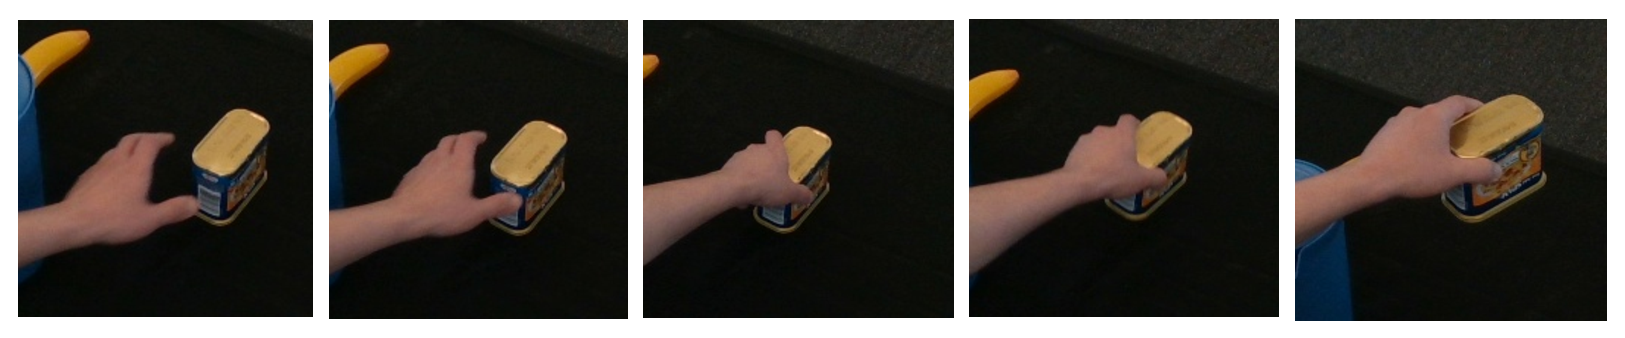
\includegraphics[width=\linewidth]{figs/1_rgb}
        \caption{Input}
    \end{subfigure}
    \hfill
    \begin{subfigure}{0.98\textwidth}
        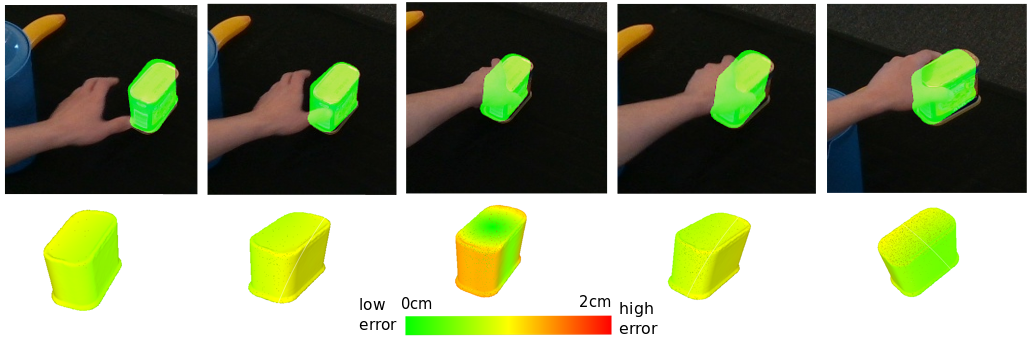
\includegraphics[width=\linewidth]{figs/1_1}
        \caption{Ours}
    \end{subfigure}
    \hfill
    \begin{subfigure}{0.98\textwidth}
        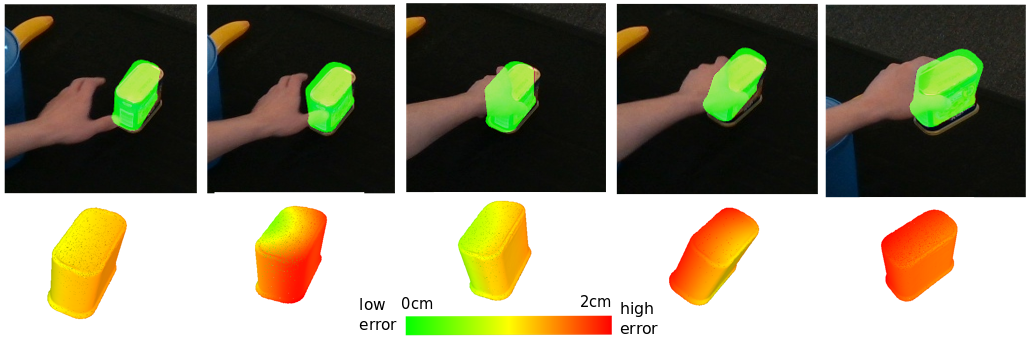
\includegraphics[width=\linewidth]{figs/1_2}
        \caption{Wang et al. \cite{wang2023deep}}
    \end{subfigure}
    \caption{Qualitative Comparison of the state-of-the-art video-based method \cite{wang2023deep} and our method. The proposed method robustly generates more stable and accurate poses over time than previous approaches. (a) are the input RGB images. (b-c) shows the rendered images using predicted object poses and colorcoded visualization of point-wise distance error.}
    \label{fig:result1}
\end{figure*}

%-------------------------------------------------------
\begin{figure*}[!ht]
    \begin{subfigure}{0.98\textwidth}
        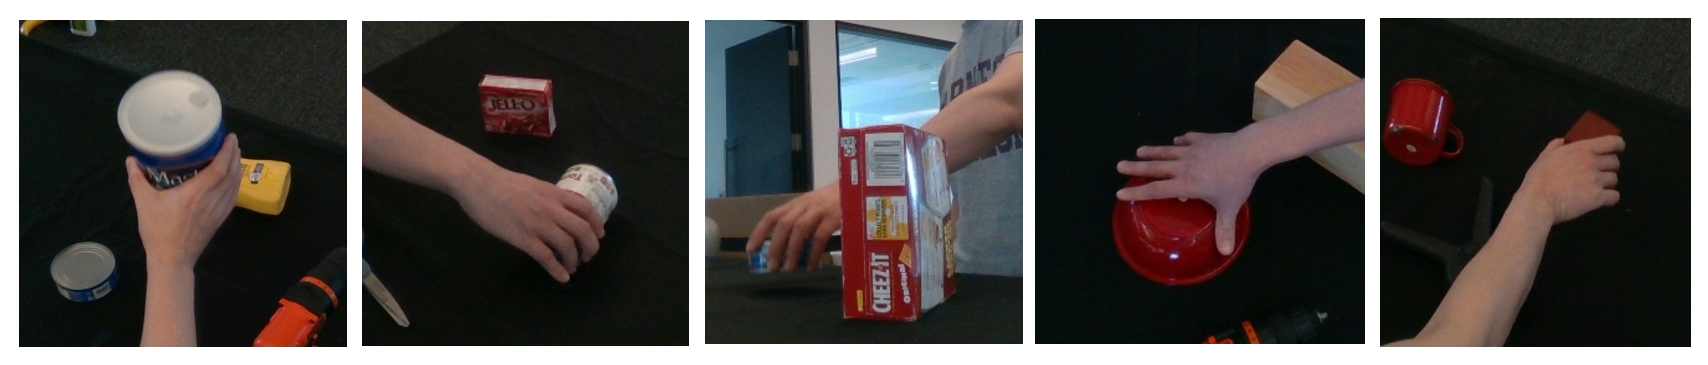
\includegraphics[width=\linewidth]{figs/2_rgb}
        \caption{Input}
    \end{subfigure}
    \hfill
    \begin{subfigure}{0.98\textwidth}
        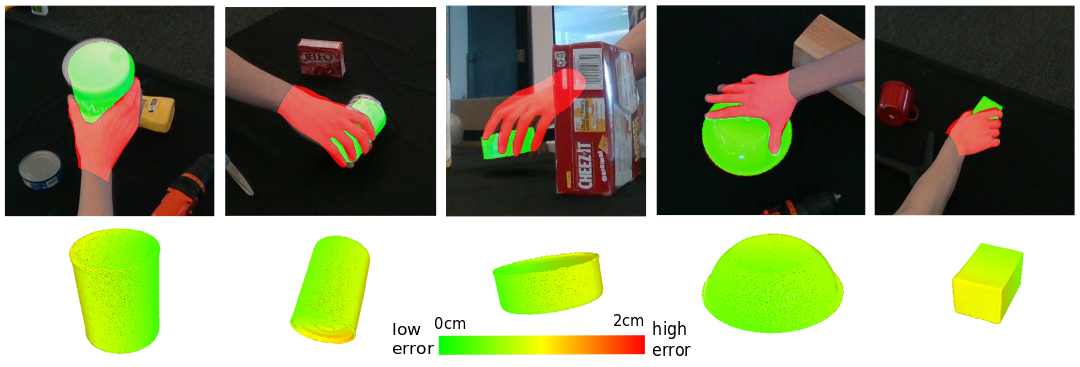
\includegraphics[width=\linewidth]{figs/2_1}
        \caption{Ours}
    \end{subfigure}
    \hfill
    \begin{subfigure}{0.98\textwidth}
        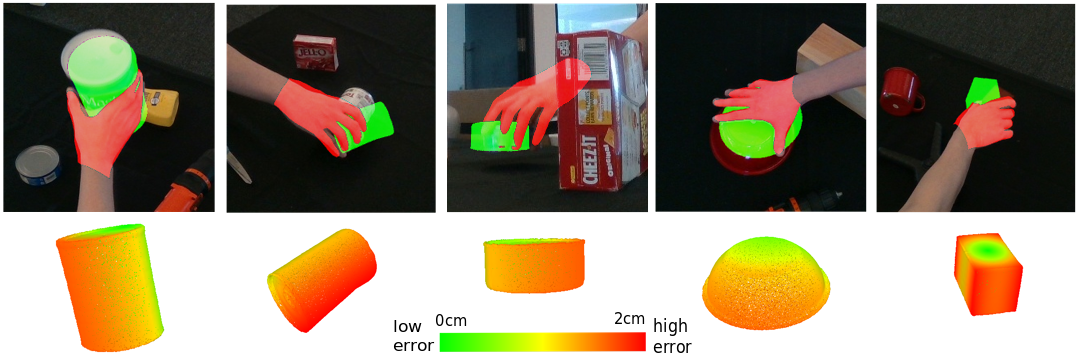
\includegraphics[width=\linewidth]{figs/2_2}
        \caption{Wang et al. \cite{wang2023deep}}
    \end{subfigure}
    \caption{Qualitative Comparison of the state-of-the-art video-based method \cite{wang2023deep}, and our method. Here we only show results on frames under heavy occlusion (frames with a visibility score \( v_i \) smaller than \( \delta = 0.5 \)). (a) are the input RGB images. (b-c) shows the rendered images using predicted object poses and colorcoded visualization of point-wise distance error.}
    \label{fig:result2}
\end{figure*}
%-------------------------------------------------------

\subsection{Evaluation Metric}
\label{sec:metric}

To evaluate the accuracy of the estimated pose \(\mathbf{\hat{P}}\) compared to the ground-truth pose \(\mathbf{\bar{P}}\) of an object model \(M\), we employ Average Distance of Model Points (ADD) metric \cite{hinterstoisser2012model}. This metric determines the average distance between corresponding vertices of the object in its ground-truth and estimated poses. Mathematically, given the ground-truth rotation \(\mathbf{\bar{R}}\) and translation \(\mathbf{\bar{t}}\), and the estimated rotation \(\mathbf{\hat{R}}\) and translation \(\mathbf{\hat{t}}\), the ADD is expressed as:

\begin{equation}
ADD = \frac{1}{m} \sum_{x \in M} \parallel (\mathbf{\bar{R}}x + \mathbf{\bar{t}}) - (\mathbf{\hat{R}}x + \mathbf{\hat{t}}) \parallel,
\end{equation}

\noindent where \(m\) represents the number of points on the object model. For symmetric objects, the ADD metric is modified to use the minimum distance between corresponding points, as described in \cite{bregier2017symmetry}. We assess the accuracy of the pose predictions using the Average Precision (AP) metric \cite{bregier2017symmetry}, where a 6D pose estimate is classified as a true positive if the ADD is within 10\% of the object's smallest bounding sphere diameter. Additionally, we report the Area Under the ADD Curve (AUC) \cite{wang2019densefusion}, which summarizes the model's performance across a range of error thresholds.

\subsection{Result}

Figures \ref{fig:result1} and \ref{fig:result2} provide a qualitative comparison of the proposed method with existing state-of-the-art methods for in-hand object pose estimation. In Figure \ref{fig:result1}, the proposed method consistently produces more stable and accurate pose predictions over time compared to the state-of-the-art video-based method \cite{wang2023deep}. In Figure \ref{fig:result2}, the comparison focuses on frames with heavy occlusion. The visibility-aware module in our approach allows the system to leverage temporal information from neighboring frames, resulting in accurate pose estimation despite the lack of clear visual cues. Both Wang et al. and Castro et al.'s methods struggle in these scenarios, as evidenced by the distorted and less accurate object poses. Our method, by contrast, maintains reliable predictions under occlusion, demonstrating the effectiveness of integrating the visibility-aware module into the spatial-temporal architecture.

%----------------------------------------------------------
\begin{table*}[h]
\caption{Quantitative results on the DexYCB \cite{chao2021dexycb}, FPHAB \cite{garcia2018first}, and HO-3D \cite{hampali2020honnotate} datasets. Single image -based methods \cite{billings2019silhonet, peng2019pvnet, wang2021gdr, castro2023crt}, and tracking methods \cite{sun2021robust, huang2021pixel, he2021ffb6d, stoiber2020sparse, stoiber2022srt3d, tian2022large, wang2023deep} are compared with our proposed method (Ours).}
\label{tab:dataset_ex}
\begin{center}
\begin{tabular}{l c c c c c c c} 
\hline
& \multicolumn{2}{c}{DexYCB} & \multicolumn{2}{c}{FPHAB} & \multicolumn{2}{c}{HO-3D} & Time \\
\hline
Method & $AUC$ & $AP$ & $AUC$ & $AP$ & $AUC$ & $AP$ & $ms$ \\  
\hline 
Billings et al. \cite{billings2019silhonet} & 54.1 & 55.2 & 56.5 & 57.4 & 55.7 & 56.2 & 35 \\

Peng et al. \cite{peng2019pvnet} & 57.6 & 58.5 & 59.1 & 60.3 & 58.3 & 59.2 & 38 \\

Wang et al.\cite{wang2021gdr} & 59.3 & 60.8 & 61.2 & 62.6 & 60.4 & 61.4 & 32 \\

Castro et al. \cite{castro2023crt} & 61.5 & 62.4 & 63.6 & 64.3 & 62.6 & 63.7 & 30 \\

\hline 

Sun et al. \cite{sun2021robust} & 60.5 & 61.4 & 63.6 & 64.2 & 61.9 & 62.6 & 87 \\

Huang et al. \cite{huang2021pixel} & 68.3 & 69.5 & 69.5 & 70.2 & 68.1 & 69.4 & 67 \\

Stoiber et al. \cite{stoiber2020sparse} & 67.2 & 67.5 & 68.4 & 69.2 & 67.9 & 68.3 & 98 \\

Stoiber et al. \cite{stoiber2022srt3d} & 71.4 & 72.8 & 73.5 & 74.3 & 71.1 & 72.2 & 87 \\

Tian et al. \cite{tian2022large} & 72.4 & 72.9 & 74.1 & 75.4 & 73.3 & 74.2 & 78 \\

Wang et al. \cite{wang2023deep} & 74.6 & 75.5 & 76.2 & 77.1 & 76.0 & 76.3 & 33 \\

Ours & \textbf{80.1} & \textbf{80.8} & \textbf{81.6} & \textbf{82.6} & \textbf{81.1} & \textbf{82.3} & 66 \\
\hline
\end{tabular}
\end{center}
\end{table*}

%-------------------------------------------------

Table \ref{tab:dataset_ex} presents the quantitative comparison of our proposed method with both single-image-based and tracking-based methods across three datasets: DexYCB \cite{chao2021dexycb}, FPHAB \cite{garcia2018first}, and HO-3D \cite{hampali2020honnotate}. The metrics used for evaluation are AUC (Area Under the ADD Curve) and AP (Average Precision). The table clearly illustrates that single-image-based methods, such as \cite{billings2019silhonet}, \cite{peng2019pvnet}, \cite{wang2021gdr}, and \cite{castro2023crt}, underperform compared to tracking-based methods, which is expected given the importance of temporal information in in-hand object pose tracking tasks. Among the tracking-based methods, \cite{wang2023deep} delivers strong performance with AUC scores of 74.6\%, 76.2\%, and 76.0\% on the DexYCB, FPHAB, and HO-3D datasets, respectively. However, our proposed method significantly outperforms all other approaches, achieving the highest AUC scores of 80.1\%, 81.6\%, and 81.1\% across these datasets. This improvement is attributed to the incorporation of transformers for spatial-temporal modeling and the visibility-aware module, which effectively handles occlusions and maintains robust pose estimation even under challenging conditions. Additionally, our method demonstrates competitive inference time, operating at 66ms per frame. Although not the fastest, it offers a well-balanced trade-off between execution speed and performance, outperforming faster but less accurate methods such as \cite{castro2023crt} and \cite{wang2021gdr}. These results validate the effectiveness of our approach in enhancing the accuracy and robustness of in-hand object pose tracking across diverse real-world scenarios.


%----------------------------------------------------------
\begin{table*}[h]
\caption{Quantitative results on the DexYCB \cite{chao2021dexycb}, FPHAB \cite{garcia2018first}, and HO-3D \cite{hampali2020honnotate} datasets. However, here we only evaluate methods on frames under heavy occlusion (frames with a visibility score \( v_i \) smaller than \( \delta = 0.5 \)). Single image-based methods \cite{billings2019silhonet, peng2019pvnet, wang2021gdr, castro2023crt}, and tracking methods \cite{sun2021robust, huang2021pixel, he2021ffb6d, stoiber2020sparse, stoiber2022srt3d, tian2022large, wang2023deep} are compared with our proposed method (Ours).}
\label{tab:occlusion_ex}
\begin{center}
\begin{tabular}{l c c c c c c c} 
\hline
& \multicolumn{2}{c}{DexYCB } & \multicolumn{2}{c}{FPHAB } & \multicolumn{2}{c}{HO-3D} & Time \\
\hline
Method & $AUC$ & $AP$ & $AUC$ & $AP$ & $AUC$ & $AP$ & $ms$ \\  
\hline 
Billings et al. \cite{billings2019silhonet} & 48.4 & 49.6 & 51.0 & 52.3 & 50.3 & 51.5 & 35 \\

Peng et al. \cite{peng2019pvnet} & 52.1 & 53.6 & 54.5 & 56.1 & 53.0 & 54.1 & 38 \\

Wang et al. \cite{wang2021gdr} & 54.8 & 54.4 & 56.0 & 57.3 & 55.4 & 56.3 & 32 \\

Castro et al. \cite{castro2023crt} & 55.2 & 56.2 & 57.0 & 57.3 & 58.1 & 58.9 & 30 \\

\hline 

Sun et al. \cite{sun2021robust} & 58.2 & 57.1 & 60.1 & 61.2 & 60.2 & 61.3 & 87 \\

Huang et al. \cite{huang2021pixel} & 63.9 & 64.8 & 64.6 & 65.0 & 63.5 & 64.6 & 67 \\

Stoiber et al.\cite{stoiber2020sparse} & 61.1 & 61.5 & 62.6 & 63.1 & 61.4 & 62.0 & 98 \\

Stoiber et al. \cite{stoiber2022srt3d} & 63.5 & 63.9 & 64.6 & 65.1 & 66.7 & 67.0 & 87 \\

Tian et al. \cite{tian2022large} & 65.0 & 65.8 & 67.7 & 68.5 & 66.8 & 67.4 & 78 \\

Wang et al. \cite{wang2023deep} & 67.3 & 68.4 & 69.1 & 70.0 & 69.7 & 69.2 & 33 \\

Ours & \textbf{78.3} & \textbf{78.5} & \textbf{79.4} & \textbf{80.1} & \textbf{79.6} & \textbf{80.8} & 66 \\
\hline
\end{tabular}
\end{center}
\end{table*}
%-------------------------------------------------

Table \ref{tab:occlusion_ex} evaluates the performance of various methods under heavy occlusion, specifically focusing on frames with a visibility score \( v_i \) smaller than \( \delta = 0.5 \). Compared to Table \ref{tab:dataset_ex} in the previous section, which evaluates overall performance, the results here reveal a key strength of our proposed method: its robustness under challenging occlusions. While most methods experience a significant drop in performance when evaluated under heavy occlusion, our method shows only a slight reduction in accuracy. For instance, on the DexYCB dataset, our method achieves an AUC of 78.3\%, compared to 80.1\% in the general evaluation from Table \ref{tab:dataset_ex}, representing a minor 1.8\% decrease. Similarly, on the FPHAB and HO-3D datasets, our method exhibits minimal reductions in AUC, with only a 2.2\% and 1.5\% decrease, respectively. In contrast, other methods suffer more substantial performance degradation under occlusion. For example, \cite{wang2023deep}, which performed well in the general evaluation, drops from 74.6\% to 67.3\% in AUC on the DexYCB dataset, representing a 7.3\% decrease. This trend is consistent across all datasets, where competing methods see larger reductions in both AUC and AP metrics. The relative stability of our method's performance highlights the effectiveness of the proposed modules, particularly the visibility-aware object pose estimation module. By dynamically adjusting pose predictions based on the visibility of the object and aggregating information from less occluded frames, our approach significantly mitigates the impact of occlusions on pose estimation accuracy. This robustness is crucial for maintaining reliable performance in real-world applications where occlusions are common, and further underscores the importance of our hybrid architecture that integrates both spatial-temporal reasoning and visibility-aware mechanisms.

\subsection{Comparison with Transformer-Based Methods}

%----------------------------------------------------------
\begin{table*}[h]
\caption{Performance comparison of our method with existing transformer-based approaches for 6D object pose estimation across three benchmark datasets. We only evaluate methods on frames under heavy occlusion (frames with a visibility score \( v_i \) smaller than \( \delta = 0.5 \)).}
\label{tab:Transformer-Based}
\begin{center}
\begin{tabular}{l c c c c c c c} 
\hline
& \multicolumn{2}{c}{DexYCB} & \multicolumn{2}{c}{FPHAB} & \multicolumn{2}{c}{HO-3D} & Time \\
\hline
Method & $AUC$ & $AP$ & $AUC$ & $AP$ & $AUC$ & $AP$ & $ms$ \\  
\hline 

Zhou et al. \cite{zhou2023deep} & 61.6 & 59.7 & 62.8 & 63.0 & 62.1 & 63.9 & 82 \\

Zhou et al. \cite{zhou2023deep} + CosyPose \cite{labbe2020cosypose} & 69.1 & 67.2 & 70.1 & 71.3 & 70.4 & 71.3 & 98 \\

Hong et al. \cite{hong2024transformer} & 61.9 & 60.2 & 63.7 & 64.3 & 63.5 & 64.2 & 86 \\

Hong et al. \cite{hong2024transformer} + CosyPose \cite{labbe2020cosypose} & 71.2 & 69.6 & 71.0 & 73.7 & 71.1 & 72.0 & 93 \\

Li et al. \cite{li2023depth} & 58.0 & 56.7 & 60.0 & 61.7 & 60.8 & 61.5 & 67 \\

Li et al. \cite{li2023depth} + CosyPose \cite{labbe2020cosypose} & 65.5 & 64.2 & 68.3 & 69.0 & 66.2 & 68.4 & 84 \\

Periyasamy et al. \cite{periyasamy2023yolopose} & 59.1 & 58.2 & 61.0 & 61.9 & 60.8 & 61.5 & 69 \\

Periyasamy et al. \cite{periyasamy2023yolopose} + CosyPose \cite{labbe2020cosypose} & 66.3 & 67.1 & 68.8 & 69.0 & 66.2 & 67.2 & 79 \\

Ours & \textbf{78.3} & \textbf{78.5} & \textbf{79.4} & \textbf{80.1} & \textbf{79.6} & \textbf{80.8} & 66 \\
\hline
\end{tabular}
\end{center}
\end{table*}

%-------------------------------------------------

Table \ref{tab:Transformer-Based} provides a detailed evaluation of transformer-based methods for 6D object pose estimation. This analysis highlights both the baseline performance of these methods and the enhancements achieved through CosyPose \cite{labbe2020cosypose} augmentation while comparing them to our proposed approach.

The transformer-based methods evaluated, including Zhou et al. \cite{zhou2023deep}, Hong et al. \cite{hong2024transformer}, Li et al. \cite{li2023depth}, and Periyasamy et al. \cite{periyasamy2023yolopose}, show promising results with AUC values ranging from 58.0\% to 63.7\% across datasets. Methods such as Zhou et al. and Hong et al. perform slightly better than others due to their use of advanced feature aggregation techniques, such as the Deep Fusion Transformer (DFTr) block and Vision Transformer (ViT) for multi-modal optimization. Despite these advancements, the absence of a dedicated mechanism to address occlusions, motion blur, and dynamic hand-object interactions significantly limits their robustness. For example, while Hong et al. achieves the best standalone performance on FPHAB (AUC: 63.7\%), its performance on more dynamic datasets like DexYCB and HO-3D remains suboptimal compared to our method.

To improve consistency across video frames, CosyPose augmentation \cite{labbe2020cosypose} was applied to each of these transformer-based methods. The process begins with the single-view transformer-based methods generating 6D object pose hypotheses. CosyPose then matches these hypotheses across different input frames to jointly estimate the camera viewpoints and the 6D poses of all objects in a single consistent scene. This augmentation significantly improves the performance of all methods. For instance, Zhou et al. \cite{zhou2023deep} achieves an AUC of 69.1\% on DexYCB after CosyPose augmentation, compared to its standalone performance of 61.6\%. Similarly, Hong et al. achieves 71.2\% AUC on DexYCB and 73.7\% AP on FPHAB after augmentation, compared to its respective standalone values of 61.9\% and 64.3\%. While CosyPose enhances pose consistency and refinement by leveraging cross-frame information, it cannot fully compensate for the limitations of the original transformer architectures, especially in handling severe occlusions and rapidly changing appearances.

Our proposed method consistently outperforms both the standalone and augmented transformer-based approaches across all datasets. On DexYCB, our method achieves an AUC of 78.3\% and AP of 78.5\%, outperforming Zhou et al. + CosyPose by a significant margin (AUC: 69.1\%, AP: 67.2\%). Similarly, on FPHAB, our approach achieves an AUC of 79.4\% and AP of 80.1\%, surpassing Hong et al. + CosyPose (AUC: 71.2\%, AP: 73.7\%) by over 8\%. On HO-3D, our method achieves an AUC of 79.6\% and AP of 80.8\%, which is 8.5\% higher than the best augmented method. These results demonstrate the effectiveness of our visibility-aware module and the Pose Transformer in addressing occlusions and dynamic variations directly within the model architecture, without requiring additional refinement stages like CosyPose.

All transformer-based methods included in this evaluation were trained using the code published by the respective authors. To ensure a fair comparison, we conducted extensive hyperparameter tuning for each method, experimenting with learning rates, batch sizes, and other critical parameters to achieve optimal performance. Training was conducted on a consistent hardware setup.

\subsection{Ablation Study}

%----------------------------------------------------------
\begin{table*}[h]
\caption{Ablation Study. $\mathcal{M}_{s}$ spatial transformer, $\mathcal{M}_{t}$ temporal transformer, $\mathcal{M}_{va}$ visibility-aware object pose estimation module.}
\label{tab:ablation_ex}
\begin{center}
\begin{tabular}{l c c c c c c c} 
\hline
& \multicolumn{2}{c}{DexYCB} & \multicolumn{2}{c}{FPHAB} & \multicolumn{2}{c}{HO-3D} & Time \\
\hline
Method & $AUC$ & $AP$ & $AUC$ & $AP$ & $AUC$ & $AP$ & $ms$ \\  
\hline 

Without Transformers & 58.2 & 57.1 & 60.1 & 61.2 & 60.2 & 61.3 & 87 \\

Without $\mathcal{M}_{t}$ and $\mathcal{M}_{s}$ & 65.7 & 66.4 & 68.5 & 68.9 & 67.2 & 68.4 & 28 \\

Without $\mathcal{M}_{s}$ & 73.7 & 74.1 & 74.2 & 75.0 & 76.3 & 77.2 & 35 \\

Without $\mathcal{M}_{t}$ & 71.2 & 72.3 & 74.9 & 76.3 & 73.5 & 74.0 & 36 \\

Without $\mathcal{M}_{va}$ & 75.1 & 77.2 & 76.5 & 76.8 & 75.6 & 76.9 & 34 \\

Ours (Full) & \textbf{80.1} & \textbf{80.8} & \textbf{81.6} & \textbf{82.6} & \textbf{81.1} & \textbf{82.3} & 66 \\
\hline
\end{tabular}
\end{center}
\end{table*}

%-------------------------------------------------

Table \ref{tab:ablation_ex} presents the results of the ablation study, which evaluates the contributions of the spatial transformer module ($\mathcal{M}_{s}$), temporal transformer module ($\mathcal{M}_{t}$), and visibility-aware object pose estimation module ($\mathcal{M}_{va}$) to the overall performance of our proposed method. The goal of this analysis is to assess the impact of each component by systematically removing them from the model and measuring the resulting performance on the DexYCB, FPHAB, and HO-3D datasets.

The results show that removing either the spatial or temporal transformers leads to a significant drop in performance. For instance, when both $\mathcal{M}_{s}$ and $\mathcal{M}_{t}$ are excluded, the AUC drops to 65.7\% on DexYCB, indicating a substantial decrease of 14.4\% compared to the full model. This highlights the importance of spatial-temporal reasoning for capturing the dynamic nature of in-hand object pose tracking. Similarly, removing only the spatial transformer ($\mathcal{M}_{s}$) results in a notable performance drop, with an AUC of 73.7\% on DexYCB, which underscores the critical role that spatial dependencies play in enhancing the model's understanding of object-hand interactions within individual frames. When the temporal transformer ($\mathcal{M}_{t}$) is excluded, the model also suffers a decline in performance across all datasets. For example, on the HO-3D dataset, the AUC decreases from 81.1\% (full model) to 73.5\%, demonstrating the essential role of temporal reasoning in improving pose estimation accuracy across video sequences. This result indicates that while spatial information is crucial, temporal dependencies are equally important for maintaining robust tracking performance over time. The visibility-aware module ($\mathcal{M}_{va}$) also plays a significant role in handling occlusions. Removing this module results in a moderate drop in performance, with the AUC on DexYCB decreasing to 75.1\%. This reduction in accuracy highlights the effectiveness of the visibility-aware mechanism in ensuring reliable pose estimation even in frames where the object is partially or fully occluded. By dynamically adjusting predictions based on object visibility and aggregating information from neighboring frames, this module enhances the model's robustness in challenging scenarios. Overall, the ablation study confirms that the combination of the spatial transformer, temporal transformer, and visibility-aware modules is critical for achieving the best performance. The full model consistently outperforms its ablated variants across all datasets, with an AUC of 80.1\% on DexYCB, 81.6\% on FPHAB, and 81.1\% on HO-3D. Despite the added complexity of integrating these components, the inference time remains competitive at 66ms, demonstrating that the proposed method offers a practical balance between accuracy and efficiency for real-time in-hand object pose tracking applications.

\subsection{Runtime Analysis and Computational Efficiency}

Our method achieves a balance between computational efficiency and accuracy, making it suitable for real-world applications. The average inference time for a single frame is 66ms, measured on a single NVIDIA RTX 2080Ti GPU, corresponding to a processing speed of approximately 15 frames per second (FPS). This runtime includes computations for both spatial and temporal transformers as well as the visibility-aware module for handling occlusions. While transformer-based architectures are inherently more computationally demanding than simpler models, our framework incorporates optimizations that reduce latency without sacrificing performance. Several factors contribute to the efficiency of our approach. The spatial transformer encoder utilizes positional embeddings and multi-head self-attention layers to process frame-wise features efficiently while maintaining a fixed computational budget. Similarly, the temporal transformer encoder integrates long-range dependencies across sequences in parallel, avoiding the iterative bottlenecks of sequential processing. The visibility-aware module further enhances computational efficiency by dynamically focusing on frames with low visibility, thereby bypassing redundant computations for highly visible frames. These optimizations collectively ensure that our model operates effectively within real-time constraints.

To further enhance runtime performance, we propose strategies such as model compression, which includes pruning and quantization to reduce the size and computation requirements of the model. For instance, lowering the precision of weights and activations to 16-bit floating point (FP16) can reduce memory usage and increase GPU throughput. Additionally, spatial and temporal transformer computations can be executed in parallel pipelines to leverage modern multi-core GPUs, minimizing latency through concurrent processing. Frame grouping into mini-batches can also benefit GPU optimizations, allowing multiple frames to be processed in parallel. Furthermore, selectively invoking the visibility-aware module only for frames with low visibility scores reduces unnecessary computation, and precomputing static spatial features for non-dynamic sequence elements can offload redundant operations.

\subsection{Limitations and Future Work}

While our approach demonstrates significant improvements in object pose tracking under occlusions, there are limitations that warrant discussion. One of the primary challenges is scalability to larger datasets. Although our method has been evaluated on benchmarks such as DexYCB, FPHAB, and HO-3D, the computational demands of transformer-based architectures may pose challenges when scaling to significantly larger datasets with higher resolution images or longer video sequences. The increased sequence length could lead to higher memory consumption and slower training times due to the quadratic complexity of attention mechanisms in transformers. Efficient adaptations, such as sparse attention mechanisms or hierarchical transformers, could be explored in future work to address this limitation.

Another limitation lies in real-time performance. While our approach achieves a processing speed of 15 FPS on an NVIDIA RTX 2080Ti GPU, this may not meet the stringent requirements of some real-time applications, particularly in resource-constrained environments or systems requiring higher frame rates. Although we have proposed strategies such as model compression, selective module invocation, and parallel processing to improve runtime efficiency, implementing and validating these optimizations in practical scenarios remains an area for future investigation.

Additionally, the reliance on labeled datasets for training and evaluation presents another limitation. Current datasets used in our experiments provide well-annotated frames for training and testing; however, real-world deployment may involve objects or environments not represented in these datasets. Exploring methods for unsupervised or semi-supervised learning could enhance the adaptability of our framework to new settings without requiring extensive labeled data.

\section{Conclusion}

In this paper, we introduced a novel framework for in-hand object pose tracking that effectively addresses the challenges posed by dynamic occlusions and rapid hand movements. By leveraging a hybrid architecture that combines the strengths of convolutional neural networks (CNNs) for spatial feature extraction with transformers for temporal reasoning, our method achieves robust and accurate pose estimation across video sequences. A key innovation of our approach is the visibility-aware module, which dynamically adjusts pose predictions based on the object's visibility, allowing the model to maintain high accuracy even under challenging conditions where portions of the object are occluded or blurred. Extensive experiments conducted on three public datasets DexYCB, FPHAB, and HO-3D demonstrate the superior performance of our method compared to existing state-of-the-art techniques. Our approach consistently outperforms these methods across various metrics, highlighting its effectiveness in both standard and occlusion-heavy scenarios. The results of the ablation studies further validate the importance of each component in our model, particularly the integration of spatial-temporal transformers and the visibility-aware mechanism, which collectively contribute to the robustness and accuracy of the pose tracking process.

Beyond achieving competitive accuracy, our method also maintains a practical balance between performance and computational efficiency, making it suitable for real-time applications in fields such as robotics, augmented reality, and human-computer interaction. The ability to accurately track objects in-hand, even under challenging conditions, opens up new possibilities for enhancing the interactivity and functionality of systems in these domains. For future work, we plan to explore the extension of our framework to handle more complex and cluttered environments, as well as its application to multi-object pose tracking scenarios. Additionally, we aim to optimize the computational aspects of our model further, enabling faster inference while preserving accuracy, thereby enhancing its applicability to real-time, resource-constrained environments. By continuing to refine and expand our approach, we hope to contribute to the development of more intelligent and adaptive systems capable of understanding and interacting with the physical world in a more sophisticated manner. \\

